\chapter{Pauli路径积分模拟}



\section{量子计算的经典模拟}
随着量子计算硬件的快速发展,量子比特规模已达到数百量级(如IBM Quantum Heron处理器)。然而,当前含噪声中等规模量子(NISQ)设备的计算保真度仍受限于退相干时间和门操作误差。在此背景下,量子计算的经典模拟技术具有多重意义:
\begin{itemize}
    \item 量子计算的经典模拟是验证量子计算硬件的有效手段。通过经典模拟,我们可以验证量子计算硬件的正确性,评估其性能,甚至优化量子算法。
    \item 突破现有量子计算硬件的规模限制。通过经典模拟,我们可以模拟更大规模的量子系统,以探索量子计算的潜在应用(如数千量子比特)。
    \item 辅助算法设计。通过经典模拟,为算法提供参数优化、误差分析等支持。
\end{itemize}
在本章中,我们将介绍量子计算的经典模拟方法,重点介绍Pauli路径积分模拟方法。


\subsection{全状态模拟}
常见的量子计算经典模拟方法包括全状态模拟,全状态模拟全状态模拟(Full-State Simulation)是量子计算经典模拟的一种直接方法,即在经典计算机上存储和演化完整的量子态向量或密度矩阵。

在纯态量子计算模型中,一个$n$量子比特的量子态可以用$2^n$维复向量表示:
\begin{equation}
    |\psi\rangle = \sum_{i=0}^{2^n-1} c_i |i\rangle,
    \quad c_i \in \mathbb{C}, \quad \sum_{i=0}^{2^n-1} |c_i|^2 = 1.
\end{equation}
在态向量模拟中,整个量子态向量被存储在计算机内存中。并在应用量子门时,通过矩阵乘法和线性代数运算来模拟量子态的演化:
\begin{equation}
    |\psi'\rangle = U |\psi\rangle,
\end{equation}
其中$U$是一个$2^n \times 2^n$的酉矩阵,表示量子门的作用。
在计算复杂度上,应用一个量子门的计算复杂度为$O(2^n)$。对于存储复杂度,一个$n$量子比特的量子态需要$2^n$个复数来存储。

对于模拟含噪声的量子计算硬件,或是模拟包含量子信道的系统,全状态模拟需要存储和操作$2^n \times 2^n$的密度矩阵:
\begin{equation}
    \rho = \sum_{i,j=0}^{2^n-1} \rho_{ij} |i\rangle\langle j|,
    \quad \rho_{ij} \in \mathbb{C},
\end{equation}
其中$\rho_{ij}$是密度矩阵的元素。在应用量子门时,密度矩阵的演化可以表示为:
\begin{equation}
    \rho' = U \rho U^\dagger.
\end{equation}
如果考虑噪声过程或量子信道,通过Kraus算符$\{K_i\}$描述量子信道的演化:
\begin{equation}
    \rho' = \sum_i K_i \rho K_i^\dagger.
\end{equation}
同样地,对于密度矩阵模拟,计算复杂度和存储复杂度也是关于qubit数目的指数级量级。

全状态模拟的主要优点是直观、易于理解,但其缺点也显而易见:存储复杂度和计算复杂度都是指数级的,因此全状态模拟只适用于小规模量子系统的模拟。对于大规模量子系统,全状态模拟的计算和存储复杂度是无法接受的。因此,我们需要寻找更高效的量子计算经典模拟方法。

\subsection{Stabilizers稳定子模拟}


一个n量子比特的纯态  $|\psi\rangle $ 被称为稳定子态,如果存在一个由n个独立、对易的Pauli算符组成的集合  $\{S_1, S_2, …, S_n\}$ ,使得:
\begin{equation}
    S_i |\psi\rangle = |\psi\rangle, \quad \forall i \in \{1, 2, …, n\}.
\end{equation}
每个生成元  $S_i$  是由单比特Pauli算符的张量积构成的算符,可以表示为:

\begin{equation}
    S_i = \alpha_i P_{i1} \otimes P_{i2} \otimes … \otimes P_{in},
\end{equation}
其中,  $\alpha_i\in\{-1,+1\}$  是相位因子,  $P_{ij}\in\{I, X, Y, Z\}$  是单比特Pauli算符。


这些算符的集合被称为  $|\psi\rangle $ 的稳定子群(Stabilizer Group),记作 $ \mathcal{S}$ 。由于这些算符是对易的,因此  $\mathcal{S}$  是Pauli群的一个阿贝尔子群。
同样的,$n$个对易的Pauli算符的集合也可以生成一个稳定子群,且该该稳定子群唯一地对应一个量子态满足$S\ket{\psi_S}=\ket{\psi_S}$对任意$S\in\mathcal{S}$成立。


例如,对于单比特态  $|0\rangle$ ,有:

\begin{equation}
    Z |0\rangle = |0\rangle.
\end{equation}
$|0\rangle$的稳定子群是 $\mathcal{S} = \{I,Z\}$ 。


一个Pauli算符可以用两个boolean值向量和一个相位因子表示:
\begin{equation}
    P = (-1)^\alpha \otimes_{i=1}^n X_i^{x_i} Z_i^{z_i},
\end{equation}
其中,$\alpha\in\{0,1\}$是相位因子,  $x_i, z_i\in\{0,1\}$  是boolean值向量。这意味着,一个Pauli算符可以用一个长度为  $2n+1$  的boolean值向量表示。因此,一个$n\times (2n+1)$的boolean值矩阵可以表示一个稳定子群的完整信息。

同时,因为Pauli算符在Clifford门作用下是闭的,任何的Clifford门构成的量子线路可以通过在作用Clifford门之后更新稳定子群的表格模拟。已知的算法可以实现以$\order{n^2}$的计算复杂度更新一次表格~\cite{PhysRevA.70.052328}。

\section{Pauli路径积分模拟}
在这一节中,我们将介绍一种高效的量子计算经典模拟方法,使用Feynman路径积分的思想,将量子线路的演化结果表示为以Pauli算符为基的路径积分。在本节中,我们将介绍Pauli路径积分模拟方法的基本原理和实现细节。

为了方便,我们假设量子线路$\mathcal{U}$包含$L$层量子门,每一层包含若干个量子门。同一层的量子门作用在不同的量子比特上,因此可以并行作用。对于真实的量子硬件,每一个门能够作用的量子比特数目是有限的,如果限制一个量子门只能作用到至多$k$个量子比特上,我们称为$k$-local量子门。对于常见的量子硬件,如超导量子比特,通常$k=2$。
%在本章中,我们暂不考虑$k$-local量子门的限制,即我们可以任意选择量子门作用的量子比特,将会在后续复杂度和误差分析中讨论这一问题。
为了方便,我们记$\mathcal{U} = \mathcal{U}_L\circ \mathcal{U}_{L-1} \cdots \mathcal{U}_1$,其中$\mathcal{U}_i$表示第$i$层的量子门复合的幺正算符。
假设$\mathcal{U}_i$包含$k_i$个量子门,则第$i$层的幺正算符$\mathcal{U}_i$可以表示为:
\begin{equation}
    \mathcal{U}_i = U_{i,1} \otimes U_{i,2} \otimes \cdots \otimes U_{i,k_i}\otimes I_{\{\supp(U_{i,1})\cup \cdots \cup \supp(U_{i,k_i})\}^c},
\end{equation}
其中$U_{i,j}$表示第$i$层第$j$个量子门,$\supp(U_{i,j})$表示$U_{i,j}$作用的量子比特集合,$I_{\{\supp(U_{i,1})\cup \cdots \cup \supp(U_{i,k_i})\}^c}$表示作用在没有被$U_{i,j}$作用的量子比特上的恒等算符。

假设量子线路$\mathcal{U}$作用在初始量子态$\rho$上,并在演化后在可观测量$O$上进行测量,我们的目标是计算量子线路$\mathcal{U}$的期望值:
\begin{equation}
    \langle O \rangle = \Tr(O \mathcal{U} \rho \mathcal{U}^\dagger).
\end{equation}
为了计算$\langle O \rangle$,我们引入Feynman路径积分的思想,将$\langle O \rangle$表示为以Pauli算符为基的路径积分:
\begin{equation}
    \langle O \rangle = \sum_{\bm{s}} f(\mathcal{U},\bm{s},O,\rho),
\end{equation}
其中$\bm{s} = (s_0, s_1, \cdots, s_L)$表示Pauli路径。
在后续的内容中,我们将介绍Pauli路径的定义和计算方法,以及如何通过Pauli路径计算$\langle O \rangle$。

\subsection{Pauli路径}
为了高效的计算量子线路的期望值,对于给定的目标线路$\mathcal{U}$,我们引入Pauli路径的概念。
Pauli路径的定义如下:

\begin{definition}
    对于一个深度为$L$的量子线路$\mathcal{U}$,其对应的Pauli路径
    \begin{equation}
        \bm{s} = (s_0, s_1, \cdots, s_L)
    \end{equation}
    是一个长度为$L+1$的序列,其中$s_i$是一个$n$比特的归一化后Pauli算符,$s_i \in \bm{P}_n=\{\frac{\mathbb{I}}{\sqrt{2}},\frac{X}{\sqrt{2}},\frac{Y}{\sqrt{2}},\frac{Z}{\sqrt{2}}\}^{\otimes n}$。
\end{definition}




我们的目标是计算$\langle O \rangle$,由式~\eqref{eq:tn:trace},我们可以将$\langle O \rangle=\Tr(O \mathcal{U} \rho \mathcal{U}^\dagger)$表示为张量网络图:
\begin{equation}
    \langle O \rangle = \Tr(O \mathcal{U} \rho \mathcal{U}^\dagger)=
    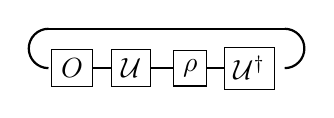
\begin{tikzpicture}[baseline=(current bounding box.center)]
        \coordinate(l)at(-0.3,0.5){};\coordinate(r)at(2.7,0.5){};
        \node[rectangle,draw] (H) at (0,0) {$O$};
        \node[rectangle,draw] (U) at (0.75,0) {$\mathcal{U}$};
        \node[rectangle,draw] (rho) at (1.5,0) {$\rho$};
        \node[rectangle,draw] (Ud) at (2.25,0) {$\mathcal{U}^\dagger$};
        \draw [thick] (H)--(U)--(rho)--(Ud) (l) -- (r);
        \draw[thick] (-0.3,0.5) arc(90:270:0.25);
        \draw[thick] (2.7,0) arc(-90:90:0.25);
    \end{tikzpicture}.
\end{equation}
因为$\mathcal{U}=\mathcal{U}_L\circ \mathcal{U}_{L-1} \cdots \mathcal{U}_1$,通过式~\eqref{eq:tn:matrix_product},我们有:
\begin{equation}
    \begin{aligned}
        \langle O \rangle = &
    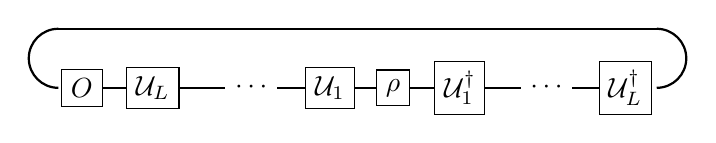
\begin{tikzpicture}[baseline=(current bounding box.center)]
        \coordinate(l)at(-0.45,0.75){};\coordinate(r)at(7.15,0.75){};
        \node[rectangle,draw] (H) at (-0.15,0) {$O$};
        \node[rectangle,draw] (Ul) at (0.75,0) {$\mathcal{U}_L$};
        \node[rectangle,draw] (Ujt) at (6.75,0) {${\mathcal{U}}_L^\dagger$};
        \node[rectangle,draw] (U1) at (3,0) {$\mathcal{U}_1$};
        \node[rectangle,draw] (U1t) at (4.65,0) {${\mathcal{U}}_1^\dagger$};
        \node[] (cdots_down) at (2,0) {$\cdots$};
        \node[] (cdots_up) at (5.75,0) {$\cdots$};
        \node[rectangle,draw] (rho) at (3.8,0) {$\rho$};
        \draw [thick] (H) -- (Ul)-- (cdots_down)--(U1)--(rho)-- (U1t) -- (cdots_up)--(Ujt) (l)--(r);
        \draw[thick] (-0.45,0.75) arc(90:270:0.75/2);
        \draw[thick] (7.15,0) arc(-90:90:0.75/2);
    \end{tikzpicture}\\
    = &
    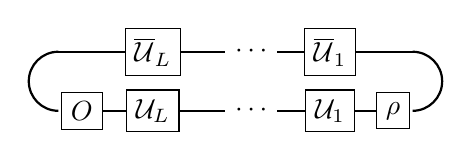
\begin{tikzpicture}[baseline=(current bounding box.center)]
        \coordinate(l)at(-0.45,0.75){};\coordinate(r)at(4.05,0.75){};
        \node[rectangle,draw] (H) at (-0.15,0) {$O$};
        \node[rectangle,draw] (Ul) at (0.75,0) {$\mathcal{U}_L$};
        \node[rectangle,draw] (Ujt) at (0.75,0.75) {$\overline{\mathcal{U}}_L$};
        \node[rectangle,draw] (U1) at (3,0) {$\mathcal{U}_1$};
        \node[rectangle,draw] (U1t) at (3,0.75) {$\overline{\mathcal{U}}_1$};
        \node[] (cdots_down) at (2,0) {$\cdots$};
        \node[] (cdots_up) at (2,0.75) {$\cdots$};
        \node[rectangle,draw] (rho) at (3.8,0) {$\rho$};
        \draw [thick] (H) -- (Ul)-- (cdots_down)--(U1)--(rho) (l) -- (Ujt) -- (cdots_up)--(U1t)--(r);
        \draw[thick] (-0.45,0.75) arc(90:270:0.75/2);
        \draw[thick] (4.05,0) arc(-90:90:0.75/2);
    \end{tikzpicture},
    \end{aligned}
\end{equation}
其中最后一个等号是因为转秩的张量网络图表示(式~\eqref{eq:tn:matrix_transpose})。


另一方面,因为$\bm{P}_n=\{\frac{\mathbb{I}}{\sqrt{2}},\frac{X}{\sqrt{2}},\frac{Y}{\sqrt{2}},\frac{Z}{\sqrt{2}}\}^{\otimes n}$构成了$n$比特的Hilbert空间的一组正交基,因此对任意的算符$T\in \mathcal{L}(\mathbb{C}^{2^n})$,我们有:
\begin{equation}
    T = \sum_{s\in \bm{P}_n} \Tr{Ts} s.
\end{equation}
表示为张量网络图:
\begin{equation}
    \sum_{s\in\bm{P}_n}
    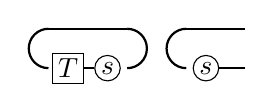
\begin{tikzpicture}[baseline=(current bounding box.center)]
      \node[draw,shape=circle,inner sep=1pt] (s1) at (1.75,0) {$s$};
      \node[draw,shape=circle,inner sep=1pt] (s0) at (0.5,0) {$s$};
      \node[rectangle,draw,inner sep=2pt] (O) at (0,0) {$T$};
      \draw[thick] (-0.25,0.5) arc(90:270:0.25);
      \draw [thick] (O)--(s0) (-0.25,0.5)--(0.75,0.5);
      \draw [thick] (2.25,0)--(s1) (1.5,0.5)--(2.25,0.5);
      \draw[thick] (1.5,0.5) arc(90:270:0.25);
      \draw[thick] (0.75,0) arc(-90:90:0.25);
    \end{tikzpicture}
    =
    \begin{tikzpicture}[baseline=(current bounding box.center)]
      \draw [thick] (O)--(1,0) (-0.25,0.5)--(1,0.5);
      \node[rectangle,draw,inner sep=2pt] (O) at (0,0) {$T$};
      \draw[thick] (-0.25,0.5) arc(90:270:0.25);
      \node[] at (1.2,0){$.$};
    \end{tikzpicture}
\end{equation}
通过多次使用上述等式,我们可以将$\langle O \rangle$表示为Pauli路径贡献的和:
\begin{equation}
    \begin{aligned}
        \langle O \rangle &= 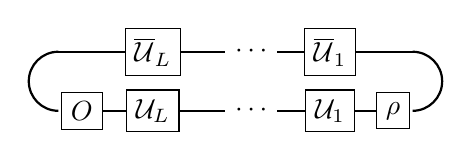
\begin{tikzpicture}[baseline=(current bounding box.center)]
            \coordinate(l)at(-0.45,0.75){};\coordinate(r)at(4.05,0.75){};
            \node[rectangle,draw] (H) at (-0.15,0) {$O$};
            \node[rectangle,draw] (Ul) at (0.75,0) {$\mathcal{U}_L$};
            \node[rectangle,draw] (Ujt) at (0.75,0.75) {$\overline{\mathcal{U}}_L$};
            \node[rectangle,draw] (U1) at (3,0) {$\mathcal{U}_1$};
            \node[rectangle,draw] (U1t) at (3,0.75) {$\overline{\mathcal{U}}_1$};
            \node[] (cdots_down) at (2,0) {$\cdots$};
            \node[] (cdots_up) at (2,0.75) {$\cdots$};
            \node[rectangle,draw] (rho) at (3.8,0) {$\rho$};
            \draw [thick] (H) -- (Ul)-- (cdots_down)--(U1)--(rho) (l) -- (Ujt) -- (cdots_up)--(U1t)--(r);
            \draw[thick] (-0.45,0.75) arc(90:270:0.75/2);
            \draw[thick] (4.05,0) arc(-90:90:0.75/2);
        \end{tikzpicture}\\
        & = \sum_{s_L \in \bm{P}_n} 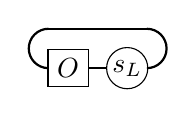
\begin{tikzpicture}[baseline=(current bounding box.center)]
            \coordinate(l)at(-0.25,0.5){};\coordinate(r)at(1,0.5){};
            \node[rectangle,draw] (H) at (0,0) {$O$};
            \node[draw,shape=circle,inner sep=1pt] (sL) at (0.75,0) {$s_L$};
            \draw [thick] (H) -- (sL) (l) -- (r);
            \draw[thick] (-0.25,0.5) arc(90:270:0.25);
            \draw[thick] (1,0) arc(-90:90:0.25);
            \end{tikzpicture}
            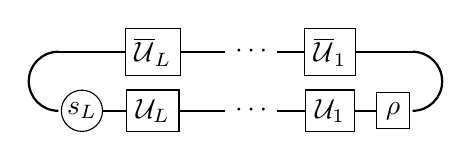
\begin{tikzpicture}[baseline=(current bounding box.center)]
                \coordinate(l)at(-0.45,0.75){};\coordinate(r)at(4.05,0.75){};
                \node[draw,shape=circle,inner sep=1pt] (H) at (-0.15,0) {$s_L$};
                \node[rectangle,draw] (Ul) at (0.75,0) {$\mathcal{U}_L$};
                \node[rectangle,draw] (Ujt) at (0.75,0.75) {$\overline{\mathcal{U}}_L$};
                \node[rectangle,draw] (U1) at (3,0) {$\mathcal{U}_1$};
                \node[rectangle,draw] (U1t) at (3,0.75) {$\overline{\mathcal{U}}_1$};
                \node[] (cdots_down) at (2,0) {$\cdots$};
                \node[] (cdots_up) at (2,0.75) {$\cdots$};
                \node[rectangle,draw] (rho) at (3.8,0) {$\rho$};
                \draw [thick] (H) -- (Ul)-- (cdots_down)--(U1)--(rho) (l) -- (Ujt) -- (cdots_up)--(U1t)--(r);
                \draw[thick] (-0.45,0.75) arc(90:270:0.75/2);
                \draw[thick] (4.05,0) arc(-90:90:0.75/2);
            \end{tikzpicture}\\
            & = \sum_{s_L,s_{L-1} \in \bm{P}_n} 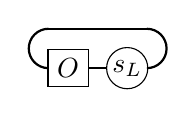
\begin{tikzpicture}[baseline=(current bounding box.center)]
                \coordinate(l)at(-0.25,0.5){};\coordinate(r)at(1,0.5){};
                \node[rectangle,draw] (H) at (0,0) {$O$};
                \node[draw,shape=circle,inner sep=1pt] (sL) at (0.75,0) {$s_L$};
                \draw [thick] (H) -- (sL) (l) -- (r);
                \draw[thick] (-0.25,0.5) arc(90:270:0.25);
                \draw[thick] (1,0) arc(-90:90:0.25);
                \end{tikzpicture}
                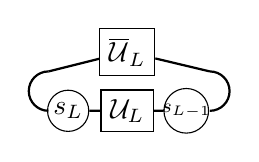
\begin{tikzpicture}[baseline=(current bounding box.center)]
                    \coordinate(l)at(-0.25,0.5){};\coordinate(r)at(1.8,0.5){};
                    \node[draw,shape=circle,inner sep=1pt] (sj) at (0.,0) {$s_L$};
                    \node[rectangle,draw] (Uj) at (0.75,0) {$\mathcal{U}_L$};
                    \node[draw,shape=circle,inner sep=-1pt] (sj1) at (1.5,0) {\scriptsize $s_{L-1}$};
                    \node[rectangle,draw] (Ujt) at (0.75,0.75) {$\overline{\mathcal{U}}_L$};
                    \draw [thick] (sj) -- (Uj) --(sj1) (l) --(Ujt)-- (r);
                    \draw[thick] (-0.25,0.5) arc(90:270:0.25);
                    \draw[thick] (1.8,0) arc(-90:90:0.25);
                  \end{tikzpicture}
                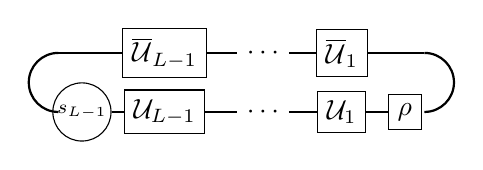
\begin{tikzpicture}[baseline=(current bounding box.center)]
                    \coordinate(l)at(-0.6,0.75){};\coordinate(r)at(4.05,0.75){};
                    \node[draw,shape=circle,inner sep=1pt] (H) at (-0.3,0) {\scriptsize $s_{L-1}$};
                    \node[rectangle,draw] (Ul) at (0.75,0) {$\mathcal{U}_{L-1}$};
                    \node[rectangle,draw] (Ujt) at (0.75,0.75) {$\overline{\mathcal{U}}_{L-1}$};
                    \node[rectangle,draw] (U1) at (3,0) {$\mathcal{U}_1$};
                    \node[rectangle,draw] (U1t) at (3,0.75) {$\overline{\mathcal{U}}_1$};
                    \node[] (cdots_down) at (2,0) {$\cdots$};
                    \node[] (cdots_up) at (2,0.75) {$\cdots$};
                    \node[rectangle,draw] (rho) at (3.8,0) {$\rho$};
                    \draw [thick] (H) -- (Ul)-- (cdots_down)--(U1)--(rho) (l) -- (Ujt) -- (cdots_up)--(U1t)--(r);
                    \draw[thick] (-0.6,0.75) arc(90:270:0.75/2);
                    \draw[thick] (4.05,0) arc(-90:90:0.75/2);
                \end{tikzpicture}\\
                &\vdotswithin{=}\\
                &=\sum_{s_0,\cdots,s_L \in \bm{P}_n}
      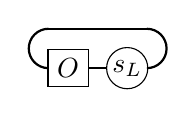
\begin{tikzpicture}[baseline=(current bounding box.center)]
        \coordinate(l)at(-0.25,0.5){};\coordinate(r)at(1,0.5){};
        \node[rectangle,draw] (H) at (0,0) {$O$};
        \node[draw,shape=circle,inner sep=1pt] (sL) at (0.75,0) {$s_L$};
        \draw [thick] (H) -- (sL) (l) -- (r);
        \draw[thick] (-0.25,0.5) arc(90:270:0.25);
        \draw[thick] (1,0) arc(-90:90:0.25);
        \end{tikzpicture}\;
      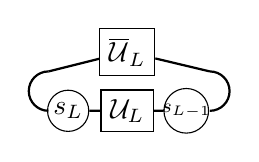
\begin{tikzpicture}[baseline=(current bounding box.center)]
        \coordinate(l)at(-0.25,0.5){};\coordinate(r)at(1.8,0.5){};
        \node[draw,shape=circle,inner sep=1pt] (sj) at (0.,0) {$s_L$};
        \node[rectangle,draw] (Uj) at (0.75,0) {$\mathcal{U}_L$};
        \node[draw,shape=circle,inner sep=-1pt] (sj1) at (1.5,0) {\scriptsize $s_{L-1}$};
        \node[rectangle,draw] (Ujt) at (0.75,0.75) {$\overline{\mathcal{U}}_L$};
        \draw [thick] (sj) -- (Uj) --(sj1) (l) --(Ujt)-- (r);
        \draw[thick] (-0.25,0.5) arc(90:270:0.25);
        \draw[thick] (1.8,0) arc(-90:90:0.25);
      \end{tikzpicture}
    \cdots
      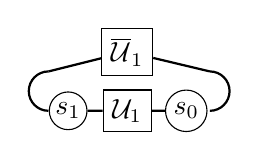
\begin{tikzpicture}[baseline=(current bounding box.center)]
        \coordinate(l)at(-0.25,0.5){};\coordinate(r)at(1.8,0.5){};
        \node[draw,shape=circle,inner sep=1pt] (sj) at (0.,0) {$s_1$};
        \node[rectangle,draw] (Uj) at (0.75,0) {$\mathcal{U}_1$};
        \node[draw,shape=circle,inner sep=1.5pt] (sj1) at (1.5,0) {$s_{0}$};
        \node[rectangle,draw] (Ujt) at (0.75,0.75) {$\overline{\mathcal{U}}_1$};
        \draw [thick] (sj) -- (Uj) --(sj1) (l) --(Ujt)-- (r);
        \draw[thick] (-0.25,0.5) arc(90:270:0.25);
        \draw[thick] (1.8,0) arc(-90:90:0.25);
      \end{tikzpicture}\;
      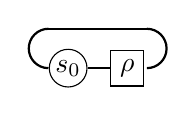
\begin{tikzpicture}[baseline=(current bounding box.center)]
        \coordinate(l)at(-0.25,0.5){};\coordinate(r)at(1,0.5){};
        \node[rectangle,draw] (rho) at (0.75,0) {$\rho$};
        \node[draw,shape=circle,inner sep=1pt] (s0) at (0.,0) {$s_0$};
        \draw [thick] (rho) -- (s0) (l) -- (r);
        \draw[thick] (-0.25,0.5) arc(90:270:0.25);
        \draw[thick] (1,0) arc(-90:90:0.25);
      \end{tikzpicture}\\
        &=\sum_{s_0,\cdots,s_L \in \bm{P}_n} \Tr{Os_L}\left(\prod_{i=1}^{L}\Tr{s_i\mathcal{U}_i s_{i-1}\mathcal{U}_i^\dagger}\right)\Tr{s_0\rho}.
    \end{aligned}
\end{equation}



对于每个具体的Pauli路径,我们可以定义该Pauli路径对应的贡献函数:

\begin{definition}
    对于一个深度为$L$的量子线路$\mathcal{U}$,和某个对应的Pauli路径$\bm{s}= (s_0, s_1, \cdots, s_L)$,初始量子态$\rho$和可观测量$O$,其贡献函数$f(\mathcal{U},\bm{s},O,\rho)$定义为:
    \begin{equation}\label{eq:pp:contribution}
        f(\mathcal{U},\bm{s},O,\rho)=\Tr{Os_L}\left(\prod_{i=1}^{L}\Tr{s_i\mathcal{U}_i s_{i-1}\mathcal{U}_i^\dagger}\right)\Tr{s_0\rho}.
    \end{equation}
\end{definition}

因此我们有:
\begin{equation}
    \langle O \rangle = \sum_{\bm{s}} f(\mathcal{U},\bm{s},O,\rho).
\end{equation}


\subsection{噪声对Pauli路径的效应}
在实际的量子计算中,由于噪声的存在,量子线路的演化会受到噪声的影响。在Pauli路径积分模拟中,我们可以通过引入噪声模型来模拟噪声对量子线路的影响。

在先前的章节中,我们已经介绍了量子信道的Kraus算符表示。对于一个量子信道$\mathcal{E}$,其Kraus算符表示为$\{K_i\}$,我们可以将量子信道$\mathcal{E}$作用在量子态$\rho$上表示为:
\begin{equation}
    \mathcal{E}(\rho) = \sum_i K_i \rho K_i^\dagger.
\end{equation}

为了方便我们可以通过张量网络图表示量子信道$\mathcal{E}$:
\begin{equation}
    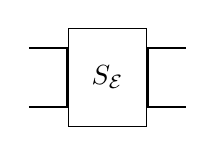
\begin{tikzpicture}[baseline=(current bounding box.center)]
        \node[draw,minimum height=1.25cm,minimum width=1cm] (s1) at (0,0) {$S_{\mathcal{E}}$};
        \draw [thick] (-1,0.375)-|(s1.west) (-1,-0.375)-|(s1.west) (s1.east)|-(1,0.375) (s1.east)|-(1,-0.375);
      \end{tikzpicture}
      \triangleq
      \sum_i
      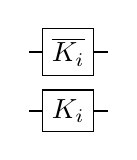
\begin{tikzpicture}[baseline=(current bounding box.center)]
        \node[draw] (s0) at (0,0) {$\overline{K_i}$};
        \node[draw] (s1) at (0,-0.75) {$K_i$};
        \draw [thick] (-0.5,0)--(s0)--(0.5,0)  (-0.5,-0.75)--(s1)--(0.5,-0.75);
      \end{tikzpicture}.
\end{equation}
算符号$S_{\mathcal{E}}$被称为量子信道Super Operator的表示~\cite{wood2011tensor},公式化地,我们有:
\begin{equation}
    S_{\mathcal{E}} = \sum_i \overline{K_i} \otimes K_i.
\end{equation}

信道$\mathcal{E}$作用在量子态$\rho$上的张量网络表示为:
\begin{equation}
    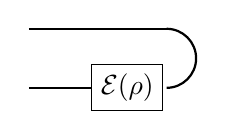
\begin{tikzpicture}[baseline=(current bounding box.center)]
        \node[draw] (rho) at (0.75,-0.75) {$\mathcal{E}(\rho)$};
        \draw [thick] (-0.5,0)--(1.25,0)  (-0.5,-0.75)--(rho);
        \draw[thick] (1.25,-0.75) arc(-90:90:0.75/2);
      \end{tikzpicture}
    =
    \sum_i
      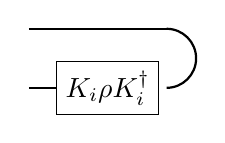
\begin{tikzpicture}[baseline=(current bounding box.center)]
        \node[draw] (rho) at (0.5,-0.75) {$K_i \rho K_i^\dagger$};
        \draw [thick] (-0.5,0)--(1.25,0)  (-0.5,-0.75)--(rho);
        \draw[thick] (1.25,-0.75) arc(-90:90:0.75/2);
      \end{tikzpicture}
      =
      \sum_i
      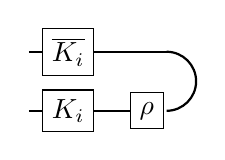
\begin{tikzpicture}[baseline=(current bounding box.center)]
        \node[draw] (s0) at (0,0) {$\overline{K_i}$};
        \node[draw] (s1) at (0,-0.75) {$K_i$};
        \node[draw] (rho) at (1,-0.75) {$\rho$};
        \draw [thick] (-0.5,0)--(s0)--(1.25,0)  (-0.5,-0.75)--(s1)--(rho);
        \draw[thick] (1.25,-0.75) arc(-90:90:0.75/2);
      \end{tikzpicture}
      =
      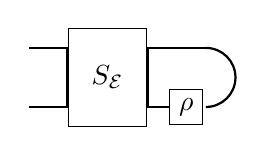
\begin{tikzpicture}[baseline=(current bounding box.center)]
        \node[rectangle,draw] (rho) at (0,-0.375) {$\rho$};
        \draw[thick] (0.25,-0.375) arc(-90:90:0.75/2);
        \node[draw,minimum height=1.25cm,minimum width=1cm] (s1) at (-1,0) {$S_{\mathcal{E}}$};
        \draw [thick] (-2,0.375)-|(s1.west) (-2,-0.375)-|(s1.west) (s1.east)|-(0.25,0.375) (s1.east)|-(rho);
      \end{tikzpicture}.
\end{equation}
在后续的讨论中,为了方便将Super Operator $S_{\mathcal{E}}$简记为$\mathcal{E}$。

我们假设量子线路$\mathcal{U}$受到噪声的影响,假设在每一层的量子门$\mathcal{U}_i$作用前和最后的测量算符$O$测量前,每个Qubit都受到噪声信道$\mathcal{N}$的作用,如图~\ref{fig:noise}所示。

\begin{figure}
    \centering
    \includegraphics[width=\textwidth]{figures/Circuit_comb.pdf}
    \caption{(a)理想的量子线路,色块代表量子门;(b)受到噪声影响的量子线路,红色的点表示噪声信道$\mathcal{N}$的作用。}
    \label{fig:noise}
\end{figure}

我们可以将受到噪声影响的量子线路表示为:
\begin{equation}
    \widehat{\mathcal{U}}(\bullet)=\mathcal{N}^{\otimes n}(\mathcal{U}_L \mathcal{N}^{\otimes n}(\cdots\mathcal{U}_1\mathcal{N}^{\otimes n}(\bullet) \mathcal{U}_1^\dagger\cdots) \mathcal{U}_L^\dagger),
\end{equation}
其中$\mathcal{N}^{\otimes n}$表示单比特的噪声信道$\mathcal{N}$作用在$n$个比特上。记$\widehat{\langle O \rangle}=\Tr(O \widehat{\mathcal{U}}(\rho))$,为含有噪声的量子线路的期望值。我们有:
\begin{equation}
    \begin{aligned}
        \widehat{\langle O \rangle}&= \Tr{ O \mathcal{N}^{\otimes n}(\mathcal{U}_L \mathcal{N}^{\otimes n}(\cdots\mathcal{U}_1\mathcal{N}^{\otimes n}(\rho) \mathcal{U}_1^\dagger\cdots) \mathcal{U}_L^\dagger)}\\
        &=\;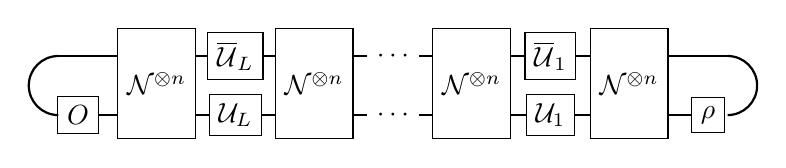
\begin{tikzpicture}[baseline=(current bounding box.center)]
          \coordinate(l)at(-0.25,0.75){};\coordinate(r)at(8.25,0.75){};
          \node[rectangle,draw] (H) at (0,0) {$O$};
          \node[rectangle,draw,minimum height=40] (Nl) at (1,0.4) {$\mathcal{N}^{\otimes n}$};
          \node[rectangle,draw] (Ul) at (2,0) {$\mathcal{U}_L$};
          \node[rectangle,draw] (Ujt) at (2,0.75) {$\overline{\mathcal{U}}_L$};
          \node[rectangle,draw,minimum height=40] (Nl1) at (3,0.4) {$\mathcal{N}^{\otimes n}$};
          \node[rectangle,draw,minimum height=40] (N1) at (5,0.4) {$\mathcal{N}^{\otimes n}$};
          \node[rectangle,draw,minimum height=40] (N0) at (7,0.4) {$\mathcal{N}^{\otimes n}$};
          \node[rectangle,draw] (U1) at (6,0) {$\mathcal{U}_1$};
          \node[rectangle,draw] (U1t) at (6,0.75) {$\overline{\mathcal{U}}_1$};
          \node[] (cdots_down) at (4,0) {$\cdots$};
          \node[] (cdots_up) at (4,0.75) {$\cdots$};
          \node[rectangle,draw] (rho) at (8,0) {$\rho$};
          \draw [thick] (H)--(H-| Nl.west) (Ul-|Nl.east)--(Ul)--(Ul-| Nl1.west) (cdots_down-|Nl1.east)--(cdots_down)--(cdots_down-| N1.west) (U1-|N1.east)--(U1)--(U1-| N0.west) (rho-|N0.east)--(rho) (l)--(l-| Nl.west) (Ujt-| Nl.east)--(Ujt)--(Ujt-| Nl1.west) (cdots_up-|Nl1.east)-- (cdots_up)--(cdots_up-| N1.west) (U1t-|N1.east)--(U1t)--(U1t-| N0.west) (r-|N0.east)--(r);
          \draw[thick] (-0.25,0.75) arc(90:270:0.75/2);
          \draw[thick] (8.25,0) arc(-90:90:0.75/2);
          \end{tikzpicture}\\
          &=\sum_{s_0,\cdots,s_L \in \bm{P}_n}
          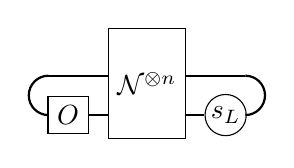
\begin{tikzpicture}[baseline=(current bounding box.center)]
            \coordinate(l)at(-0.25,0.5){};\coordinate(r)at(2.25,0.5){};
            \node[rectangle,draw] (H) at (0,0) {$O$};
            \node[rectangle,draw,minimum height=40] (N) at (1,0.4) {$\mathcal{N}^{\otimes n}$};
            \node[draw,shape=circle,inner sep=1pt] (sL) at (2,0) {$s_L$};
            \draw [thick] (H)--(H-| N.west) (sL-|N.east)--(sL) (l)--(l-| N.west) (r-|N.east)--(r);
            \draw[thick] (-0.25,0.5) arc(90:270:0.25);
            \draw[thick] (2.25,0) arc(-90:90:0.25);
            \end{tikzpicture}\;
          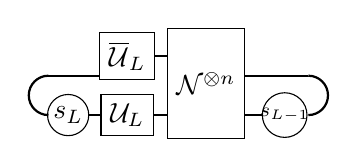
\begin{tikzpicture}[baseline=(current bounding box.center)]
            \coordinate(l)at(-0.25,0.5){};\coordinate(r)at(3.05,0.5){};
            \node[draw,shape=circle,inner sep=1pt] (sj) at (0.,0) {$s_L$};
            \node[rectangle,draw] (Uj) at (0.75,0) {$\mathcal{U}_L$};
            \node[draw,shape=circle,inner sep=-1pt] (sj1) at (2.75,0) {\scriptsize $s_{L-1}$};
            \node[rectangle,draw] (Ujt) at (0.75,0.75) {$\overline{\mathcal{U}}_L$};
            \node[rectangle,draw,minimum height=40] (N) at (1.75,0.4) {$\mathcal{N}^{\otimes n}$};
            \draw [thick] (sj)--(Uj)--(Uj-| N.west) (sj1-|N.east)--(sj1) (l) --(l-|Ujt.west) (Ujt)--(Ujt-| N.west) (r-|N.east)-- (r);
            \draw[thick] (-0.25,0.5) arc(90:270:0.25);
            \draw[thick] (3.05,0) arc(-90:90:0.25);
          \end{tikzpicture}
        \cdots
          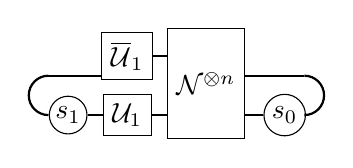
\begin{tikzpicture}[baseline=(current bounding box.center)]
            \coordinate(l)at(-0.25,0.5){};\coordinate(r)at(3,0.5){};
            \node[draw,shape=circle,inner sep=1pt] (sj) at (0.,0) {$s_1$};
            \node[rectangle,draw] (Uj) at (0.75,0) {$\mathcal{U}_1$};
            \node[draw,shape=circle,inner sep=1.5pt] (sj1) at (2.75,0) {$s_{0}$};
            \node[rectangle,draw] (Ujt) at (0.75,0.75) {$\overline{\mathcal{U}}_1$};
            \node[rectangle,draw,minimum height=40] (N) at (1.75,0.4) {$\mathcal{N}^{\otimes n}$};
            \draw [thick] (sj)--(Uj)--(Uj-| N.west) (sj1-|N.east)--(sj1) (l) --(l-|Ujt.west) (Ujt)--(Ujt-| N.west) (r-|N.east)-- (r);
            \draw[thick] (-0.25,0.5) arc(90:270:0.25);
            \draw[thick] (3,0) arc(-90:90:0.25);
          \end{tikzpicture}\;
          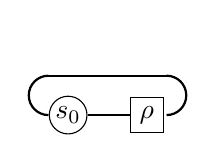
\begin{tikzpicture}[baseline=(current bounding box.center)]
            \coordinate(l)at(-0.25,0.5){};\coordinate(r)at(1.25,0.5){};
            \node[rectangle,draw] (rho) at (1,0) {$\rho$};
            \node[rectangle,draw,minimum height=40,opacity=0] (N) at (1,0.4) {$\mathcal{N}^{\otimes n}$};
            \node[draw,shape=circle,inner sep=1pt] (s0) at (0.,0) {$s_0$};
            \draw [thick] (rho)--(s0) (l)--(r);
            \draw[thick] (-0.25,0.5) arc(90:270:0.25);
            \draw[thick] (1.25,0) arc(-90:90:0.25);
          \end{tikzpicture}\\
          &=\Tr{O\mathcal{N}^{\otimes n}(s_L)}\Tr{s_L\mathcal{U}_L \mathcal{N}^{\otimes n}(s_{L-1})\mathcal{U}_L^\dagger}\cdots\Tr{s_1\mathcal{U}_1 \mathcal{N}^{\otimes n}(s_{0})\mathcal{U}_1^\dagger}\Tr{s_0\rho}.
    \end{aligned}
\end{equation}
于是我们可以定义含有噪声的Pauli路径的贡献函数:

\begin{definition}
    对于一个深度为$L$的含噪量子线路$\widehat{\mathcal{U}}$,和某个对应的Pauli路径$\bm{s}= (s_0, s_1, \cdots, s_L)$,初始量子态$\rho$和可观测量$O$,其贡献函数$f(\mathcal{U},\bm{s},O,\rho)$定义为:
    \begin{equation}
        \hat{f}(\mathcal{U},\bm{s},O,\rho)=\Tr{O\mathcal{N}^{\otimes n}(s_L)}
        \left(\prod_{i=1}^{L}\Tr{s_i\mathcal{U}_i \mathcal{N}^{\otimes n}(s_{i-1})\mathcal{U}_i^\dagger}\right)\Tr{s_0\rho},
    \end{equation}
    其中$\mathcal{U}$表示含噪声的量子线路$\widehat{\mathcal{U}}$的理想(无噪声)部分。
\end{definition}


假设系统中的噪声是单比特Pauli噪声,如式~\eqref{eq:pauli_noise}所示,Pauli噪声信道$\mathcal{N}$可以表示为$\mathcal{N}(\rho) = (1-p_x-p_y-p_z)\rho + p_x X\rho X + p_y Y\rho Y + p_z Z\rho Z$。将Pauli算符$X$、$Y$、$Z$和$I$是单位算符代入Pauli噪声信道$\mathcal{N}$,我们可以得到Pauli噪声信道$\mathcal{N}$对Pauli算符的作用:
\begin{equation}
    \begin{aligned}
        \mathcal{N}(I) &= I,\\
        \mathcal{N}(X) &= (1-2p_y-2p_z)X,\\
        \mathcal{N}(Y) &= (1-2p_x-2p_z)Y,\\
        \mathcal{N}(Z) &= (1-2p_x-2p_y)Z.
    \end{aligned}
\end{equation}
因此我们有:
\begin{equation}
    \begin{aligned}
        \mathcal{N}^{\otimes n}(s_i)= &\otimes_{j=1}^{n}\mathcal{N}(s_{i,j})\\
        =&(1-2p_y-2p_z)^{\abs{s_i}_X}(1-2p_x-2p_z)^{\abs{s_i}_Y}(1-2p_x-2p_y)^{\abs{s_i}_Z}s_i,
    \end{aligned}
\end{equation}
其中$\abs{s_i}_X$、$\abs{s_i}_Y$、$\abs{s_i}_Z$分别表示Pauli算符$s_i$中$\frac{X}{2},\frac{Y}{2},\frac{Z}{2}$的数量。因此我们可以将含噪声的Pauli路径的贡献函数用以下引理表示:
\begin{lemma}\label{lemma:noise}
    对于一个深度为$L$的含噪声量子线路$\widehat{\mathcal{U}}$,和某个对应的Pauli路径$\bm{s}= (s_0, s_1, \cdots, s_L)$,初始量子态$\rho$和可观测量$O$,在单比特Pauli噪声信道$\mathcal{N}$下,其含噪贡献函数$\hat{f}(\mathcal{U},\bm{s},O,\rho)$和理想无噪声贡献函数$f(\mathcal{U},\bm{s},O,\rho)$满足:
    \begin{equation}
        \hat{f}(\mathcal{U},\bm{s},O,\rho)=\left(1-2p_y-2p_z\right)^{\abs{\bm{s}}_X}\left(1-2p_x-2p_z\right)^{\abs{\bm{s}}_Y}\left(1-2p_x-2p_y\right)^{\abs{s}_Z}f(\mathcal{U},\bm{s},O,\rho),
    \end{equation}
    其中$\abs{\bm{s}}_P$表示整个Pauli路径$\bm{s}$中Pauli算符$P\in \{\frac{X}{2},\frac{Y}{2},\frac{Z}{2}\}$的数量(为了简化表示,我们将Pauli算符的系数$\frac{1}{2}$省略)。即
    \begin{equation}
        \abs{\bm{s}}_P = \sum_{i=0}^{L}\abs{s_i}_P.
    \end{equation}
\end{lemma}


由引理~\ref{lemma:noise},可以根据噪声的类型定义与噪声相关的Pauli路径的Hamming Weight如下:
\begin{definition}
    对于一个深度为$L$的含噪声量子线路$\widehat{\mathcal{U}}$,和某个对应的Pauli路径$\bm{s}= (s_0, s_1, \cdots, s_L)$,在由概率$p_x,p_y,p_z$定义的单比特Pauli噪声信道$\mathcal{N}$下,其与噪声关联的Hamming Weight定义为:
    \begin{equation}\label{eq:noise_hamming_weight}
        \abs{\bm{s}}_{\mathcal{N}} = \begin{cases} 
            \abs{\bm{s}}_Y+\abs{\bm{s}}_Z, & \text{如果$\{p_x,p_y,p_z\}$中只有$p_x\neq 0$} \\
            \abs{\bm{s}}_X+\abs{\bm{s}}_Z, & \text{如果$\{p_x,p_y,p_z\}$中只有$p_y\neq 0$} \\
            \abs{\bm{s}}_X+\abs{\bm{s}}_Y, & \text{如果$\{p_x,p_y,p_z\}$中只有$p_z\neq 0$} \\
            \abs{\bm{s}}_X + \abs{\bm{s}}_Y + \abs{\bm{s}}_Z, & \text{如果有$\{p_x,p_y,p_z\}$中至少有两个元素非0}
        \end{cases}
    \end{equation}
\end{definition} 

设$\gamma\triangleq \min\{p|{p \in \{p_x,p_y,p_z\},p\neq 0}\}$为噪声信道$\mathcal{N}$中非零概率的最小值。由引理~\ref{lemma:noise},我们可以得到含噪声的Pauli路径的贡献函数$\hat{f}(\mathcal{U},\bm{s},O,\rho)$与理想无噪声的Pauli路径的贡献函数$f(\mathcal{U},\bm{s},O,\rho)$之间的关系:
\begin{equation}
    \abs{\hat{f}(\mathcal{U},\bm{s},O,\rho)} \leq \gamma^{\abs{\bm{s}}_{\mathcal{N}}} \abs{f(\mathcal{U},\bm{s},O,\rho)}.
\end{equation}

\begin{figure}
    \centering
    \includegraphics[width=\textwidth]{figures/noise_path.pdf}
    \caption{噪声对Pauli路径贡献函数$f$的效应。}
    \label{fig:noise}
\end{figure}

图~\ref{fig:noise}给出了噪声对Pauli路径的贡献函数$f$效应的示意图。在无噪声的理想情况下,Pauli路径的贡献函数$f$由半透明的背景区域表示。在含有噪声的情况下,Pauli路径的贡献函数$\hat{f}$由实体的区域表示。在含有噪声的情况下,Pauli路径的贡献函数$\hat{f}$的绝对值随着与噪声关联的Hamming Weight的增加而被指数级地抑制。因为Pauli路径的个数是$4^{L(n+1)}$,其中$n$是量子比特的数量,$L$是量子线路的深度。
为了高效的模拟量子线路的期望值,在含有噪声的情况下,我们可以通过对Pauli路径的贡献函数进行有效的截断,只保留与噪声关联的Hamming Weight较小的Pauli路径,从而减少计算量。
截断的部分在图~\ref{fig:noise}中用灰色区域表示。

具体的,我们可以定义一个与噪声关联的Hamming Weight的阈值$M$,只保留与噪声关联的Hamming Weight小于等于$M$的Pauli路径的贡献函数,即:
\begin{equation}
    \widetilde{\langle O \rangle} = \sum_{\abs{\bm{s}}_{\mathcal{N}}\leq M} \hat{f}(\mathcal{U},\bm{s},O,\rho).
\end{equation}
$\widetilde{\langle O \rangle}$给出了含有噪声的量子线路的期望值$\widehat{\langle O \rangle}$的一个近似值。

\subsection{OBPPP算法}
在本节中,我们将介绍一种基于Pauli路径积分模拟的量子线路期望值计算算法——可观测量在Pauli路径下的反向传播算法(Observable's Back-Propagation on Pauli Path,OBPPP)。OBPPP算法通过计算低weight的Pauli路径的贡献函数,实现了对含有噪声的量子线路的期望值的高效计算。

算法的计算复杂度包含两个部分:Pauli路径的枚举和每个Pauli路径的贡献函数的计算,分别记为$C_s$和$C_f$。假设一共有$N_M$个Pauli路径的Hamming Weight小于等于$M$且拥有非平凡的贡献函数,则OBPPP算法的计算复杂度为$O(C_s+N_M(C_f))$。

其中$C_f$是计算一个Pauli路径的贡献函数的计算复杂度也包含三个部分:和初态相关的$\tr(\rho s_0)$的计算、和观测量相关的$\tr(Os_L)$的计算和中间量子门的计算$\prod\tr(s_i\mathcal{U}_i s_{i-1}\mathcal{U}_i^\dagger)$。这三部分的计算复杂度分别记为$C_{f\rho}$、$C_{fO}$和$C_{f\mathcal{U}}$。
因此$C_f = C_{f\rho}+C_{fO}+C_{f\mathcal{U}}$。

在后续的章节中,我们将详细介绍在一些具体的线路模型中$C_{f\mathcal{U}}$的计算复杂度。在本章中,我们将重点介绍$C_{f\rho}$、$C_{fO}$和$C_s$的计算复杂度,以及$N_M$的估计。

\subsubsection{$C_{f\rho}$的估计}
为了能高效的将初态$\rho$存储在计算机中,我们需要对初态$\rho$添加一些合理的假设。否则存储一个$n$量子比特的初态$\rho$需要$2^{2n}$个复数,这是不可行的。一个合理的假设是初态$\rho$是一个稀疏的密度矩阵,即:
\begin{definition}
    一个$n$量子比特的密度矩阵$\rho$是一个稀疏的密度矩阵,如果它的非零元素的数量是多项式级别的,即
    \begin{equation}
        \rho=\sum_{a,b} \rho_{a,b}\ketbra{a}{b},
    \end{equation}
    其中$\rho_{a,b}$是复数,$\ket{a}$和$\ket{b}$是$n$量子比特计算基态,$a,b\in \{0,1\}^n$。
    且$\rho_{a,b}$中非零元素的数量是多项式级别的,即$\abs{\{(\rho_{a,b},a,b)\mid \rho_{a,b}\neq 0\}}=\poly(n)$。
\end{definition}
对于许多常见的量子算法,如量子变分算法~\cite{peruzzo2014variational}、量子近似优化算法~\cite{farhi2014quantum}、Shor算法~\cite{shor1994algorithms}、Grover算法~\cite{grover1996fast}等,它们的初态都是计算基态,因此是稀疏的密度矩阵假设是合理的。对于这种稀疏的密度矩阵,我们可以通过存储非零元素的位置和值来高效的存储初态$\rho$。

在稀疏的密度矩阵假设下,$C_{f\rho}=O(\poly(n))$。这是因为:
对于$\rho$中的每个元素$\rho_{a,b}\ketbra{a}{b}$,$\Tr{s_0  (\rho_{a,b}\ketbra{a}{b})}$可以通过以下公式计算:
\begin{equation}\label{ap:eq:component_of_input}
\Tr{s_0  (\rho_{a,b}\ketbra{a}{b})}=\rho_{a,b} \bra{b}s_0 \ket{a}=\rho_{a,b} \prod_{j=1}^n \bra{b}_j (s_0)|_j \ket{a}_j,
\end{equation}
其中$|_j$表示限制算符在第$j$个量子比特上的限制,$\ket{\cdot}_j$表示$\ket{\cdot}$的第$j$个分量。

通过式~\eqref{ap:eq:component_of_input},$\Tr{s_0  (\rho_{a,b}\ketbra{a}{b})}$可以在时间(空间)复杂度为$\order{n}$的情况下计算。通过稀疏性假设,$\Tr{s_0 \rho}$可以在时间(空间)复杂度为$\mathrm{Poly}(n)$的情况下计算。因此,$C_{f\rho}=O(\poly(n))$。
 

算法的核心是如何高效的枚举出与噪声关联的Hamming Weight小于等于$M$的Pauli路径。对于每个给定的Pauli路径$\bm{s}$,其贡献函数$\hat{f}(\mathcal{U},\bm{s},O,\rho)$可以通过式~\eqref{eq:pp:contribution}计算。

\subsubsection{$C_{fO}$的估计}
对于和观测量$O$相关的$\Tr(Os_L)$的计算,同样的为了使得观测量$O$能够被高效的输入计算机,我们需要对观测量$O$添加一些合理的假设。在常见的量子算法中,观测量$O$通常是一些Pauli算符的线性组合,即:
\begin{equation}
    O = \sum_{i=1}^{N_O} c_i P_i,
\end{equation}
其中$c_i$是实数,$P_i$是n比特的Pauli算符。
一个合理的假设是观测量$O$是一个Pauli稀疏的观测量,即:
\begin{definition}
    一个$n$量子比特的观测量$O$是一个Pauli稀疏的观测量,如果它的非零元素的数量是多项式级别的,即
    \begin{equation}
        O=\sum_{i=1}^{N_O} c_i P_i,
    \end{equation}
    其中$c_i$是实数,$P_i$是n比特的Pauli算符。
    且$N_O$是多项式级别的,即$N_O=\poly(n)$。
\end{definition}
对于Pauli稀疏的观测量$O$,我们可以通过使用一个树状结构来存储观测量$O$中的Pauli算符和其对应的系数。
树中的每个节点分配一个Pauli算符。树的叶节点对应一个唯一的Pauli串,并存储$O$的相应系数值。
例如,考虑观测量$O=1 X_0+1 Z_1+0.5 X_0X_1$,它可以表示为图~\ref{fig:trie}所示的树。

\begin{figure}[htbp]
    \centering
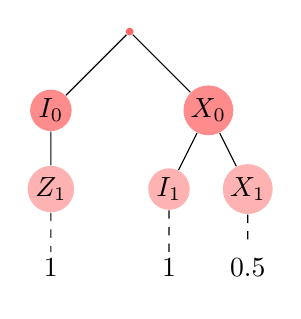
\begin{tikzpicture}
  [level distance=10mm,
   every node/.style={fill=red!60,circle,inner sep=1pt},
   level 1/.style={sibling distance=20mm,nodes={fill=red!45}},
   level 2/.style={sibling distance=10mm,nodes={fill=red!30}},
   level 3/.style={dashed,sibling distance=5mm,nodes={fill=red!0}}],
  \node[minimum size=0.01cm] { }
     child {node {$I_0$}
       child {node {$Z_1$}
       child {node {$1$}}
       }
     }
     child {node {$X_0$}
       child {node {$I_1$}
       child {node {$1$}}}
       child {node {$X_1$}
       child {node {$0.5$}}}
     };
\end{tikzpicture}
\caption{观测量$O=1 X_0+1 Z_1+0.5 X_0X_1$的树表示。}\label{fig:trie}
\end{figure}

因此,我们可以利用树状数据结构以时间复杂度$\order{n}$计算$\Tr{O s_L}$,并以空间复杂度$\mathrm{Poly}(n)$存储树。
在观测量Pauli稀疏的假设下,可以得到$C_{fO}=O(\poly(n))$。



\subsubsection{$C_s$和$N_M$的估计}

在本节中,我们将介绍如何高效的枚举出与噪声关联的Hamming Weight小于等于$M$且拥有非平凡贡献函数的Pauli路径,并估计满足条件的Pauli路径的个数$N_M$。具体的讲,需要枚举出以下集合:
\begin{equation}
    \mathcal{S}_M = \left\{ \bm{s} \mid \abs{\bm{s}}_{\mathcal{N}}\leq M, \hat{f}(\mathcal{U},\bm{s},O,\rho)\neq 0 \right\}.
\end{equation}
$N_M$是$\mathcal{S}_M$的元素个数。


在此,为了方便的估计,定义在量子线路中$\mathcal{U}$中每个门的最大可分裂的Pauli算符的数量为$N_{\text{max}}$:
\begin{definition}
    对于一个深度为$L$的量子线路$\mathcal{U}$,假设其门集合为$\{\mathcal{U}_{i,j}\}$。定义$\mathcal{U}$的门最大可分裂的Pauli算符的数量为$N_{\text{max}}$:
    \begin{equation}
        N_{\text{max}} = \max_{i,j,s}\abs{ \left\{ s'\mid \tr(s' U^\dagger_{i,j}s U_{i,j})\neq 0 \right\}},
    \end{equation}
    其中$s$和$s'$是Pauli算符,$\tr$表示Pauli算符的迹。 
\end{definition}
在后续的章节中,将估计对一些具体的线路模型中$N_{\text{max}}$的值。在本章中,将假设$N_{\text{max}}$是一个变量。

因为对于含有$n$个qubits,深度为$L$的量子线路$\mathcal{U}$,其Pauli路径的数量是$4^{L(n+1)}$。因此先枚举再筛选的方法会带来指数级的计算复杂度,在实际应用中是不可行的。因此,我们需要设计一种高效的枚举方法。

可观测量在Pauli路径下的反向传播算法正是我们对此问题的解决方案。与一般模拟算法随时间进程从初始态开始模拟的方式不同,OBPPP算法在Heisenberg图景下模拟量子线路的演化。OBPPP算法的核心思想是从观测量$O$开始,逆向的模拟量子线路的演化,直到初态$\rho$。在这个过程中,OBPPP算法会维护一个Pauli路径的集合,这个集合包含了与噪声关联的Hamming Weight小于等于$M$且拥有非平凡贡献函数的Pauli路径。OBPPP算法的示意图如图~\ref{fig:obppp}所示,左侧包含$O$的方块表示观测量$O$,算法从观测量$O$开始,逆向的模拟量子线路的演化,每个连线表示着一个Pauli路径,连线的颜色表示着Pauli路径的与噪声关联的Hamming Weight,更深的颜色表示更大的Hamming Weight。在逆向演化的过程中,Pauli算符随着Pauli路径反向传播,直到初态$\rho$。在传播的过程中,Pauli路径会发生分裂,生成更多的Pauli路径,Hamming Weight也会随着演化的过程而逐渐增加。随着传播的深入,算法会截断与噪声关联的Hamming Weight大于$M$的Pauli路径,用虚线表示。

\begin{figure}[htbp]
    \centering
    \includegraphics[width=0.7\textwidth]{figures/obppp.png}
    \caption{OBPPP算法的示意图。}
    \label{fig:obppp}
\end{figure}

首先回顾与噪声关联的Hamming Weight的定义,由式~\eqref{eq:noise_hamming_weight}给出。
